\documentclass[tikz, border=10pt]{standalone}
\usepackage{tikz}
\usepackage[sfdefault]{roboto}
\usepackage[T1]{fontenc}
\usetikzlibrary{shapes.misc, positioning, arrows.meta, fit, calc}

\begin{document}

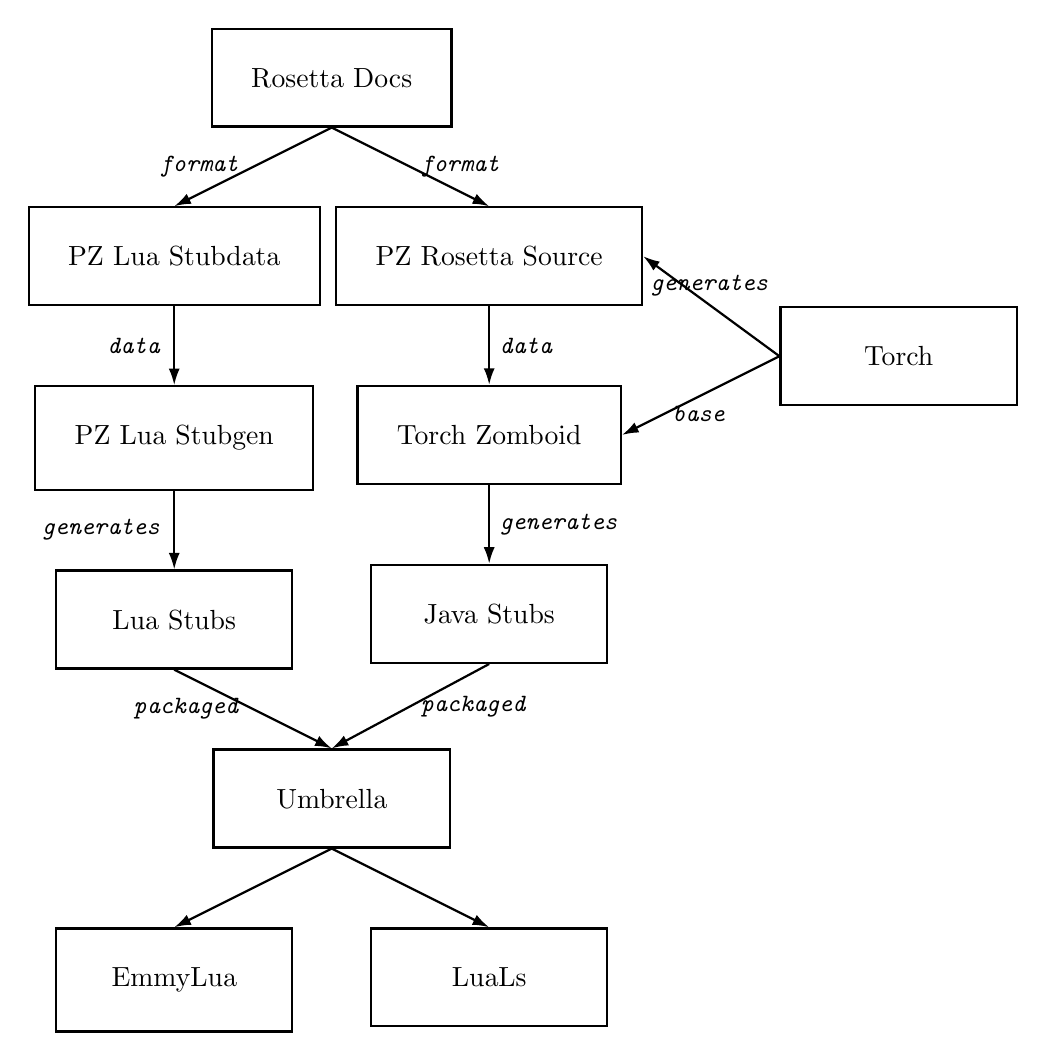
\begin{tikzpicture}[
    node distance=0.3cm,
    box/.style={rectangle, draw, thick, minimum width=3cm, inner sep=0.5cm},
    func/.style={font=\ttfamily\small, inner sep=0.15cm},
    arrow/.style={-{Latex[length=6pt, width=4pt]}, thick},
]

%% NODES
    % rosetta docs
    \node[box] (rosetta_doc) {Rosetta Docs};

    % data
    \node[box, below=1.0cm of rosetta_doc, xshift=-2cm] (pz_lua_stubdata) {PZ Lua Stubdata};
    \node[box, below=1.0cm of rosetta_doc, xshift=2cm] (pz_rosetta_source) {PZ Rosetta Source};

    % torch
    \node[box, below=1.0cm of pz_rosetta_source] (torch_zomboid) {Torch Zomboid};
    \node[box, right=2cm of torch_zomboid, yshift=1cm] (torch) {Torch};

    % generator
    \node[box, below=1.0cm of pz_lua_stubdata] (pz_lua_stubgen) {PZ Lua Stubgen};

    % stubs
    \node[box, below=1.0cm of pz_lua_stubgen] (lua_stubs) {Lua Stubs};
    \node[box, below=1.0cm of torch_zomboid] (java_stubs) {Java Stubs};

    % Umbrella
    \node[box, below=1.0cm of lua_stubs, xshift=2cm] (umbrella) {Umbrella};

    \node[box, below=1.0cm of umbrella, xshift=-2cm] (emmylua) {EmmyLua};
    \node[box, below=1.0cm of umbrella, xshift=2cm] (luals) {LuaLs};



%% CONNECTIONS
    % torch
    \draw[arrow] (torch.west) -- node[below, font=\ttfamily\small] {\textit{base}} (torch_zomboid.east);

    % data -> generator
    \draw[arrow] (pz_lua_stubdata.south) -- node[left, font=\ttfamily\small] {\textit{data}} (pz_lua_stubgen.north);
    \draw[arrow] (pz_rosetta_source.south) -- node[right, font=\ttfamily\small] {\textit{data}} (torch_zomboid.north);

    \draw[arrow] (torch.west) -- node[above, font=\ttfamily\small] {\textit{generates}} (pz_rosetta_source.east);

    % rosetta docs -> data
    \draw[arrow] (rosetta_doc.south) -- node[left, font=\ttfamily\small] {\textit{format}} (pz_lua_stubdata.north);
    \draw[arrow] (rosetta_doc.south) -- node[right, font=\ttfamily\small] {\textit{format}} (pz_rosetta_source.north);

    % generator -> stubs
    \draw[arrow] (pz_lua_stubgen.south) -- node[left, font=\ttfamily\small] {\textit{generates}} (lua_stubs.north);
    \draw[arrow] (torch_zomboid.south) -- node[right, font=\ttfamily\small] {\textit{generates}} (java_stubs.north);

    % Umbrella
    \draw[arrow] (lua_stubs.south) -- node[left, font=\ttfamily\small] {\textit{packaged}} (umbrella.north);
    \draw[arrow] (java_stubs.south) -- node[right, font=\ttfamily\small] {\textit{packaged}} (umbrella.north);

    \draw[arrow] (umbrella.south) -- (emmylua.north);
    \draw[arrow] (umbrella.south) -- (luals.north);

\end{tikzpicture}

\end{document}
